\documentclass[t, screen, aspectratio=43]{beamer}
\usepackage[T1]{fontenc}
\usepackage[utf8]{inputenc}
\usepackage{epsf}
\usepackage{graphicx}
\usepackage{geometry}
\usepackage{tabularx}
\usepackage[table]{colortbl}
\usepackage{xcolor}
\usepackage{soul}
\usepackage[normalem]{ulem}
\usepackage{tikz}
\usepackage{subcaption}
% Use the NTNU-temaet for beamer 
% \usetheme[style=ntnu|simple|vertical|horizontal, 
%     language=bm|nn|en, 
%     smalltitle, 
%     city=all|trondheim|alesund|gjovik]{ntnu2017}
\usetheme[style=helvet,language=en]{ntnu2017}

\usepackage[english]{babel}
\usepackage[style=numeric,backend=biber,natbib=false,sorting=none]{biblatex}

\title[Short title]{Ultra-Low Power PLL for Wake-up Receiver Applications}
\subtitle{Specialization Project Progress - 9th Week}
\author[C Nielsen]{Cole Nielsen}
\institute[NTNU]{Department of Electronic Systems, NTNU}
\date{18 October 2019 (Calendar week 43)}
%\date{} % To have an empty date

\addbibresource{example.bib} % Add bibliography database

% Set the reference style to numeric.
% See here: http://tex.stackexchange.com/questions/68080/beamer-bibliography-icon
\setbeamertemplate{bibliography item}[text] 

% Set bibliography fonts to a small size.
\renewcommand*{\bibfont}{\footnotesize}




\begin{document}

\begin{frame}
	\titlepage%
\end{frame}

% Alternatively, special title page command to get a different background
% \ntnutitlepage

% #############################################################################
% Timeline
% #############################################################################
\begin{frame}
	\frametitle{\color{red} Old Timeline}
	\begin{table}[htb!]
		\tiny
		\centering
		\vspace{-1em}
		\def\arraystretch{1.5}		
		\setlength\arrayrulewidth{0.75pt}
		\setlength{\tabcolsep}{1em} % for the horizontal padding
		\begin{tabular}{|l|l|l|l|}
			\hline 
			\rule[-1ex]{0pt}{2.5ex} \cellcolor{gray!40}\textbf{Week} & \cellcolor{gray!40}\textbf{Dates} &\cellcolor{gray!40}\textbf{Tasks} & \cellcolor{gray!40}\textbf{Outcomes}\\ 
			\hline 
			\rule[-1ex]{0pt}{2.5ex} \cellcolor{red!20}\textbf{36}& \cellcolor{red!20}2.9 - 8.9 & \cellcolor{red!20}Review PLL Design & \cellcolor{red!20}Refreshed Knowledge\\ 
			\hline 
			\rule[-1ex]{0pt}{2.5ex} \cellcolor{red!20}\textbf{37}& \cellcolor{red!20}9.9 - 15.9 & \cellcolor{red!20}Modeling/simulation (set up) & \cellcolor{red!20}--\\ 
			\hline 
			\rule[-1ex]{0pt}{2.5ex} \cellcolor{red!20}\textbf{38}& \cellcolor{red!20}16.9 - 22.9 & \cellcolor{red!20}Modeling/simulation &\cellcolor{red!20}TDC/DCO Requirements\\ 
			\hline 
			\rule[-1ex]{0pt}{2.5ex} \cellcolor{red!20}\textbf{39}& \cellcolor{red!20}23.9 - 29.9& \cellcolor{red!20}Modeling/simulation& \cellcolor{red!20}Loop Filter/Digital Algorithms\\ 
			\hline 
			\rule[-1ex]{0pt}{2.5ex} \cellcolor{red!20}\textbf{40}& \cellcolor{red!20}30.9 - 6.10& \cellcolor{red!20}Modeling/simulation& \cellcolor{red!20}{Loop filter, DCO, TDC, calibration}\color{black}\\ 
			\hline 
			\rule[-1ex]{0pt}{2.5ex} \cellcolor{red!20}\textbf{41}&\cellcolor{red!20}7.10 - 13.10&\cellcolor{red!20}Circuit Research &\cellcolor{red!20}DCO/Divider topologies, Ideal Virtuoso implementation\\ 
			\hline 
			\rule[-1ex]{0pt}{2.5ex} \cellcolor{red!20}\textbf{42}&\cellcolor{red!20}14.10 - 20.10&\cellcolor{red!20}Circuit Research &\cellcolor{red!20}TDC/other topologies\\ 
			\hline 
			\rule[-1ex]{0pt}{2.5ex} \color{red}\cellcolor{green!20}\textbf{43}&\color{red}\cellcolor{green!20}21.10 - 27.10&\color{red}\cellcolor{green!20}Circuit Implementation&\color{red}\cellcolor{green!20}Digital logic (schematic)\\ 
			\hline 
			\rule[-1ex]{0pt}{2.5ex} \color{red}\textbf{44}& \color{red}28.10 - 3.11& \color{red}Circuit Implementation& \color{red}DCO (schematic)\\ 
			\hline 
			\rule[-1ex]{0pt}{2.5ex} \color{red}\textbf{45}& \color{red}4.11 - 10.11& \color{red}Circuit Implementation& \color{red}Divider/other (schematic)\\ 
			\hline 
			\rule[-1ex]{0pt}{2.5ex} \color{red}\textbf{46}& \color{red}11.11 - 17.11& \color{red}Circuit Implementation (TDC)& \\ 
			\hline 
			\rule[-1ex]{0pt}{2.5ex} \color{red}\textbf{47}& \color{red}18.11 - 24.11& \color{red}Circuit Implementation (TDC)& \color{red}TDC (schematic)\\ 
			\hline 
			\rule[-1ex]{0pt}{2.5ex} \color{red}\textbf{48}& \color{red}25.11 - 1.12& \color{red}Full Circuit testing & \color{red}Testbenches, find bugs, design fixes\\ 
			\hline 
			\rule[-1ex]{0pt}{2.5ex} \color{red}\textbf{49}& \color{red}2.12 - 8.12& \color{red}Full Circuit testing& \color{red}Design Fixes/iteration\\ 
			\hline 
			\rule[-1ex]{0pt}{2.5ex} \color{red}\textbf{50}& \color{red}9.12 - 15.12& \color{red}--& \color{red}--\\ 
			\hline 
		\end{tabular}
		\begin{flushleft}\textbf{Legend:} \colorbox{red!20}{\textbf{Done}} \colorbox{green!20}{\textbf{Current}}  \colorbox{blue!20}{\textbf{Revised}}
		% *I will write the report simultaneously with the work.
		\end{flushleft}
		% \caption{Assigned specifications for branch line hybrid design.}
		% \label{asgn_specs}
	\end{table}   
\end{frame}


\begin{frame}
	\frametitle{New Timeline}
	\begin{table}[htb!]
		\tiny
		\centering
		\vspace{-1em}
		\def\arraystretch{1.5}		
		\setlength\arrayrulewidth{0.75pt}
		\setlength{\tabcolsep}{1em} % for the horizontal padding
		\begin{tabular}{|l|l|l|l|}
			\hline 
			\rule[-1ex]{0pt}{2.5ex} \cellcolor{gray!40}\textbf{Week} & \cellcolor{gray!40}\textbf{Dates} &\cellcolor{gray!40}\textbf{Tasks} & \cellcolor{gray!40}\textbf{Outcomes}\\ 
			\hline 
			\rule[-1ex]{0pt}{2.5ex} \cellcolor{red!20}\textbf{36}& \cellcolor{red!20}2.9 - 8.9 & \cellcolor{red!20}Review PLL Design & \cellcolor{red!20}Refreshed Knowledge\\ 
			\hline 
			\rule[-1ex]{0pt}{2.5ex} \cellcolor{red!20}\textbf{37}& \cellcolor{red!20}9.9 - 15.9 & \cellcolor{red!20}Modeling/simulation (set up) & \cellcolor{red!20}--\\ 
			\hline 
			\rule[-1ex]{0pt}{2.5ex} \cellcolor{red!20}\textbf{38}& \cellcolor{red!20}16.9 - 22.9 & \cellcolor{red!20}Modeling/simulation &\cellcolor{red!20}TDC/DCO Requirements\\ 
			\hline 
			\rule[-1ex]{0pt}{2.5ex} \cellcolor{red!20}\textbf{39}& \cellcolor{red!20}23.9 - 29.9& \cellcolor{red!20}Modeling/simulation& \cellcolor{red!20}Loop Filter/Digital Algorithms\\ 
			\hline 
			\rule[-1ex]{0pt}{2.5ex} \cellcolor{red!20}\textbf{40}& \cellcolor{red!20}30.9 - 6.10& \cellcolor{red!20}Modeling/simulation& \cellcolor{red!20}{Loop filter, DCO, TDC, calibration}\color{black}\\ 
			\hline 
			\rule[-1ex]{0pt}{2.5ex} \cellcolor{red!20}\textbf{41}&\cellcolor{red!20}7.10 - 13.10&\cellcolor{red!20}Circuit Research &\cellcolor{red!20}DCO/Divider topologies\\ 
			\hline 
			\rule[-1ex]{0pt}{2.5ex} \cellcolor{red!20}\textbf{42}&\cellcolor{red!20}14.10 - 20.10&\cellcolor{red!20}Circuit Research &\cellcolor{red!20}TDC/other topologies\\ 
			\hline 
			\rule[-1ex]{0pt}{2.5ex} \cellcolor{green!20}\textbf{43}&\cellcolor{green!20}21.10 - 27.10&\cellcolor{green!20}Spur analysis, filter automation &\cellcolor{green!20} \\ 
			\hline 
			\rule[-1ex]{0pt}{2.5ex} \textbf{44}& 28.10 - 3.11& Filter automation, variance analysis& DSP round-off optimization\\ 
			\hline 
			\rule[-1ex]{0pt}{2.5ex} \textbf{45}& 4.11 - 10.11& Variation analysis, flicker noise & Histograms/yield estimates\\ 
			\hline 
			\rule[-1ex]{0pt}{2.5ex} \textbf{46}& 11.11 - 17.11& Real DCO sensitivity, TDC/divider jitter& Simlate ring-DCO in Virtuoso\\ 
			\hline 
			\rule[-1ex]{0pt}{2.5ex} \textbf{47}& 18.11 - 24.11& PLL + Radio simulation& BER estimate\\ 
			\hline 
			\rule[-1ex]{0pt}{2.5ex} \textbf{48}& 25.11 - 1.12& Agglomerate into cohesive framework & (I have an Exam on 30.11)\\ 
			\hline 
			\rule[-1ex]{0pt}{2.5ex} \textbf{49}& 2.12 - 8.12& Finish framework, report writing& \\ 
			\hline 
			\rule[-1ex]{0pt}{2.5ex} \textbf{50}& 9.12 - 15.12& Report writing& Complete before 15.12\\ 
			\hline 
		\end{tabular}
		\begin{flushleft}\textbf{Legend:} \colorbox{red!20}{\textbf{Done}} \colorbox{green!20}{\textbf{Current}}  \colorbox{blue!20}{\textbf{Revised}}
		% *I will write the report simultaneously with the work.
		\end{flushleft}
		% \caption{Assigned specifications for branch line hybrid design.}
		% \label{asgn_specs}
	\end{table}   
\end{frame}


% #############################################################################
% This week
% #############################################################################

\begin{frame}
	\frametitle{(New) Timeline Tasks}
	\begin{block}{This week}
		\begin{itemize}
			\footnotesize
			\item \textbf{Spur analysis:}
			\begin{itemize}
				\footnotesize
				\item Implemented phase noise reference spur analysis.
			\end{itemize} 
			\item \textbf{Filter automation}:
			\begin{itemize}
				\footnotesize
				\item Now that project is a a PLL simulation framework, improve filter design
				\item Automatic filter design was lacking
				\begin{itemize}
					\scriptsize
					\item Previously required manual selection of gain parameter, so not fully automated
					\item Now fully automated.
				\end{itemize}				
				\item Improve resemblence of generated filter to prototype filter.
			\end{itemize} 
			\item \textbf{Improved code-reusability}:
			\begin{itemize}
				\footnotesize
				\item Previously used several mostly independent scripts, now all use same core code for simulating PLL.
				\item PLL core code configured with dictionary.
			\end{itemize} 
		\end{itemize}    
	\end{block}
\end{frame}

% #############################################################################
% sim/modeling approach
% #############################################################################

\begin{frame}
	\frametitle{Reference spur analysis}
	\vspace{-0.7em}
	\begin{block}{Reference spur simulation}
		% \vspace{-0.5em}
		% \center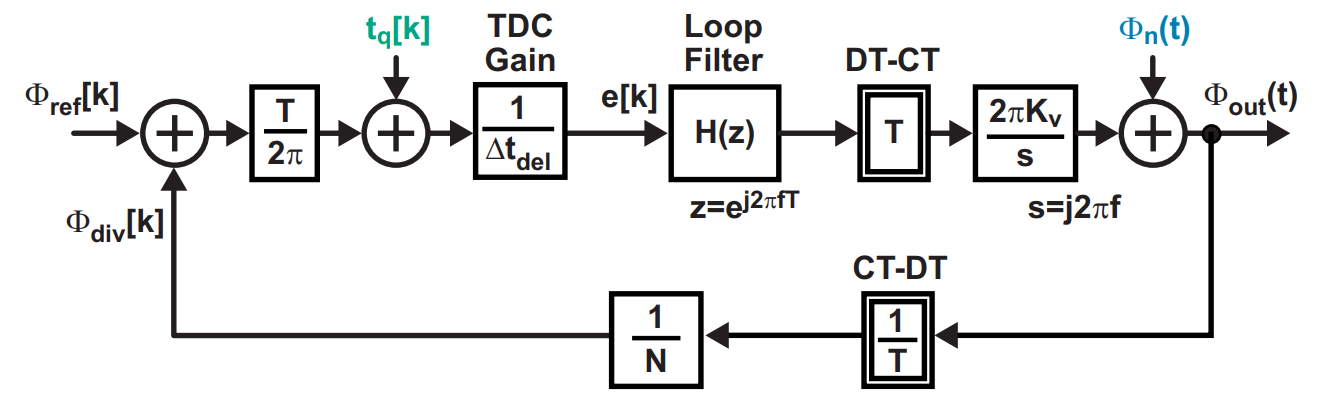
\includegraphics[width=0.6\textwidth, angle=0]{pll_loop.png}
		\begin{itemize}
			\scriptsize
			\item Due to discrete time/tuning nature of DCO, spurs are produced in the phase noise spectrum at offsets from the carrier that are multiples of the reference frequency.
			\item In steady state, relatively few changes occur in oscillator tuning word (ca. 1 LSB in 100's or 1000's of reference cycles).
			\item Time between OTW changes in steady state is relatively stochastic compared to reference cycle frequency, so spurs should be quite small in these conditions.
			\vspace{-0.5em}
		\begin{figure}[htb!]
	        \centering
	        \begin{subfigure}{.4\textwidth}
	            \centering
	            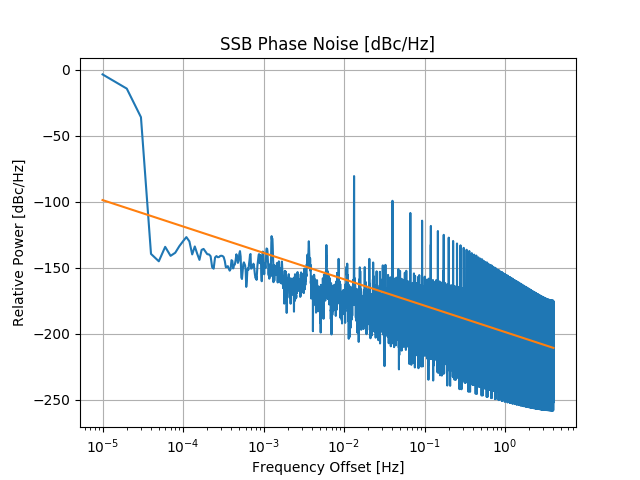
\includegraphics[width=0.9\linewidth]{pn_spurs.png}
	            \caption{\scriptsize Severe spurs.}
	            \label{fig:rosc_3stg_cir}
	        \end{subfigure}%
	        \begin{subfigure}{.4\textwidth}
	            \centering
	            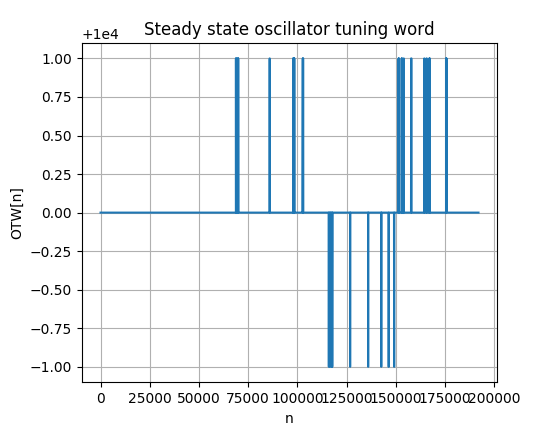
\includegraphics[width=0.9\linewidth]{otw_ss.png}
	            \caption{\scriptsize OTW in steady state.}
	            \label{fig:rosc_3stg_wave}
	        \end{subfigure}
	        % \caption{Approximate model for ring oscillator inverter delay cell.}
	        \label{fig:rosc_3stg}
	    \end{figure}
		\end{itemize} 
	\end{block}
\end{frame}

\begin{frame}
	\frametitle{Reference spur analysis}
	\begin{block}{Simulation}
		\begin{itemize}
			\scriptsize
			\item Had to rewrite phase domain simulation to support oversampling. Now simulate twice:
			\begin{itemize}
				\tiny
				\item Once sampled at the reference frequency with long span to capture low frequency phase noise.
				\item Once oversampled sampled with short span to capure reference spurs.
				\item Results are combined, with about 10x faster run-time than a single simulation capturing the same frequency range in plot (b) below.
			\end{itemize} 
		\end{itemize} 
		\vspace{-1em}
		\begin{figure}[htb!]
	        \centering
	        \begin{subfigure}{.4\textwidth}
	            \centering
	            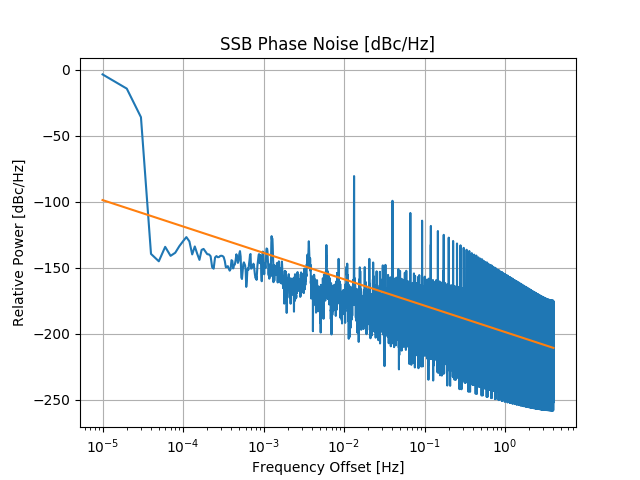
\includegraphics[width=0.9\linewidth]{pn_spurs.png}
	            \caption{\scriptsize Severe spurs.}
	            \label{fig:rosc_3stg_cir}
	        \end{subfigure}%
	        \begin{subfigure}{.4\textwidth}
	            \centering
	            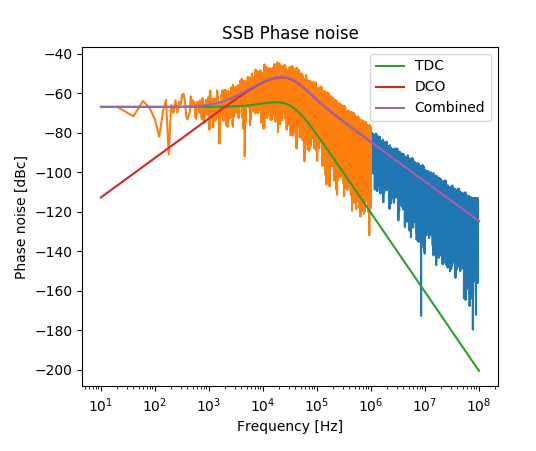
\includegraphics[width=0.9\linewidth]{stitched_pn.png}
	            \caption{\scriptsize Simulated PLL spurs (none).}
	            \label{fig:rosc_3stg_wave}
	        \end{subfigure}
	        % \caption{Approximate model for ring oscillator inverter delay cell.}
	        \label{fig:rosc_3stg}
	    \end{figure}
	\end{block}
\end{frame}

\begin{frame}
	\frametitle{Reference spur analysis}
	\vspace{-0.7em}
	\begin{block}{Simulation}
		% \vspace{-0.5em}
		% \center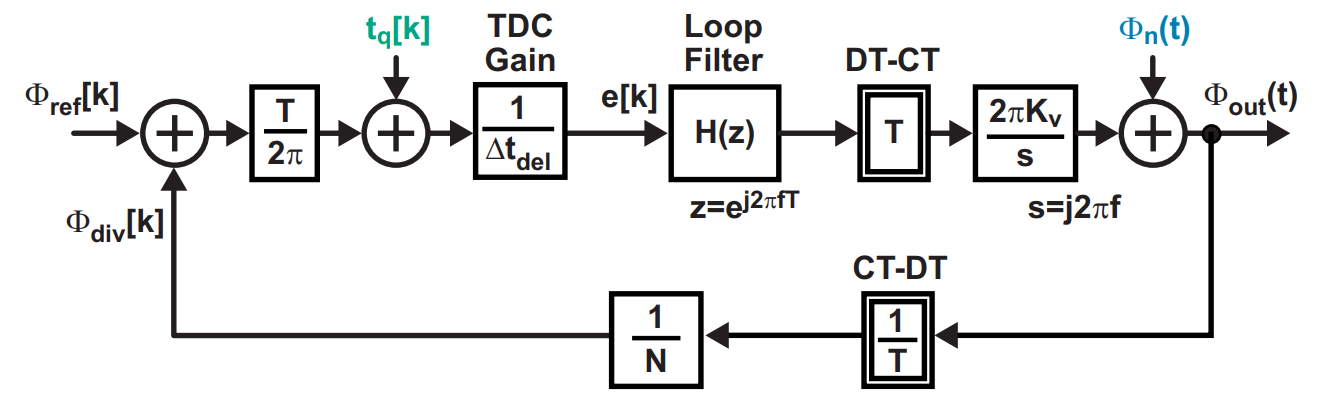
\includegraphics[width=0.6\textwidth, angle=0]{pll_loop.png}
		\begin{itemize}
			\scriptsize
			\item It does not appear spurs will be an issue in this PLL design. They are not measureable under the current assumed PLL design parameters.
			\item Generally, the DCO resolution should be high enough and the rate of change of the OTW is small enough where not much power is pushed into the reference spurs for an integer-N PLL design.
		\end{itemize} 
	\end{block}
\end{frame}


\begin{frame}
	\frametitle{Filter automation}
	\begin{block}{Deficiencies}
		\begin{itemize}
			\scriptsize
			\item Old automated filter design was a "quick and dirty" approach. 
			\begin{itemize}
				\scriptsize
				\item High/low frequency response was not well optimized. At frequencies near the loop bandwidth frequency, peaking was not well controlled.
				\item Most phase noise power is integrated in frequencies near to the loop bandwidth frequency, so excessive peaking is a bad problem.
			\end{itemize}	
		\end{itemize} 
		\vspace{-1em}
		\begin{figure}[htb!]
	        \centering
	        \begin{subfigure}{.4\textwidth}
	            \centering
	            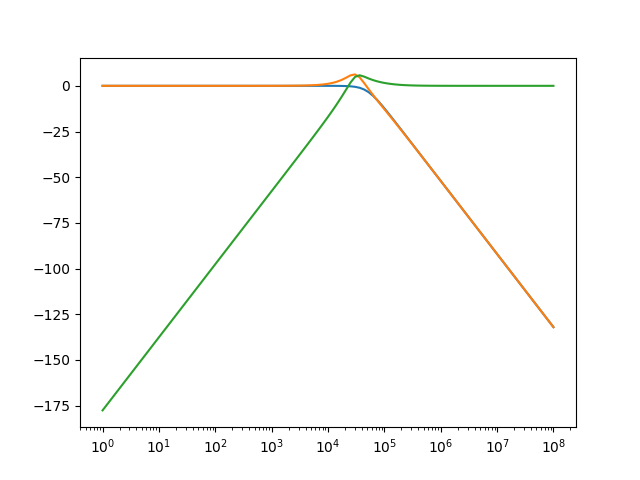
\includegraphics[width=0.9\linewidth]{old_g.png}
	            \caption{\scriptsize Optimized by old method.}
	            \label{fig:rosc_3stg_cir}
	        \end{subfigure}%
	        \begin{subfigure}{.4\textwidth}
	            \centering
	            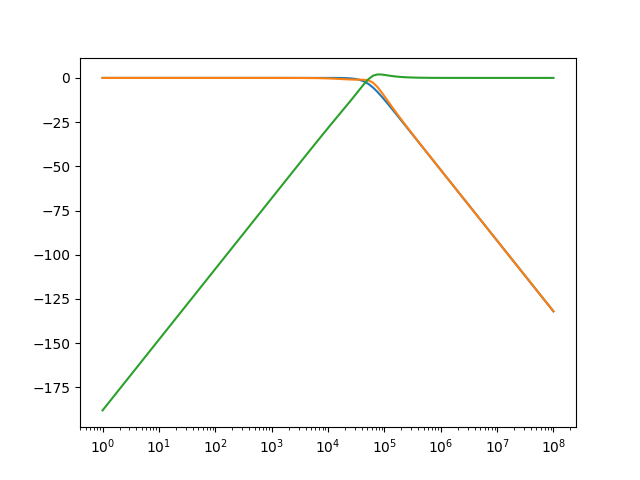
\includegraphics[width=0.9\linewidth]{better_g.png}
	            \caption{\scriptsize Optimized by new method.}
	            \label{fig:rosc_3stg_wave}
	        \end{subfigure}
	        % \caption{Approximate model for ring oscillator inverter delay cell.}
	        \label{fig:rosc_3stg}
	    \end{figure}
	\end{block}
\end{frame}

\begin{frame}
	\frametitle{Filter automation}
	\begin{block}{New approach}
		\begin{itemize}
			\scriptsize
			\item Old approach optimized the following PLL open loop transfer function for poles/zero and parameter K (put into closed loop configuration):
		\scriptsize	
		\begin{equation}
			A(s) = \frac{K}{s^2}\cdot\frac{(s/\omega_z + 1)}{(s/\omega_p + 1)}
		\end{equation}	
			\item The parameter K has very a small rate of change compared to the pole/zero frequencies, so in gradient descent little optimization occurs to K.
			\item If the desired prototype transfer function is:
		\scriptsize	
		\begin{equation}
			G(s) = \frac{\omega_n^2}{s^2 + 2\zeta \omega_n s + \omega_n^2}
		\end{equation}	
		It turns out for the tail roll-off to be the same at high frequency:
		\end{itemize} 
		\scriptsize	
		\begin{equation}
			K = \frac{\omega_z\omega_n^2}{\omega_p}
		\end{equation}	
	\end{block}
\end{frame}

\begin{frame}
	\frametitle{Filter automation}
	\begin{block}{New approach}
		\begin{itemize}
			\scriptsize
			\item Now to find the optimized loop filter parameters, a loop is run where:
			\begin{itemize}
				\tiny
				\item The pole/zero are optimized with gradient descent for a fixed K.
				\item The aforementioned equation for K is used to update K based on the optimized pole/zero
			\end{itemize} 
			\item The above is repeated until convergence.
		\end{itemize}
	\end{block}
\end{frame}



\begin{frame}
	\frametitle{Code-resuability}
	\begin{block}{More generic PLL simulation engine}
		\begin{itemize}
			\scriptsize
			\item Made generic engine to simulate integer-N PLL, configured with a dictionary.
			\item Less code fragmentation everything now uses same core.
		\end{itemize}	
		\center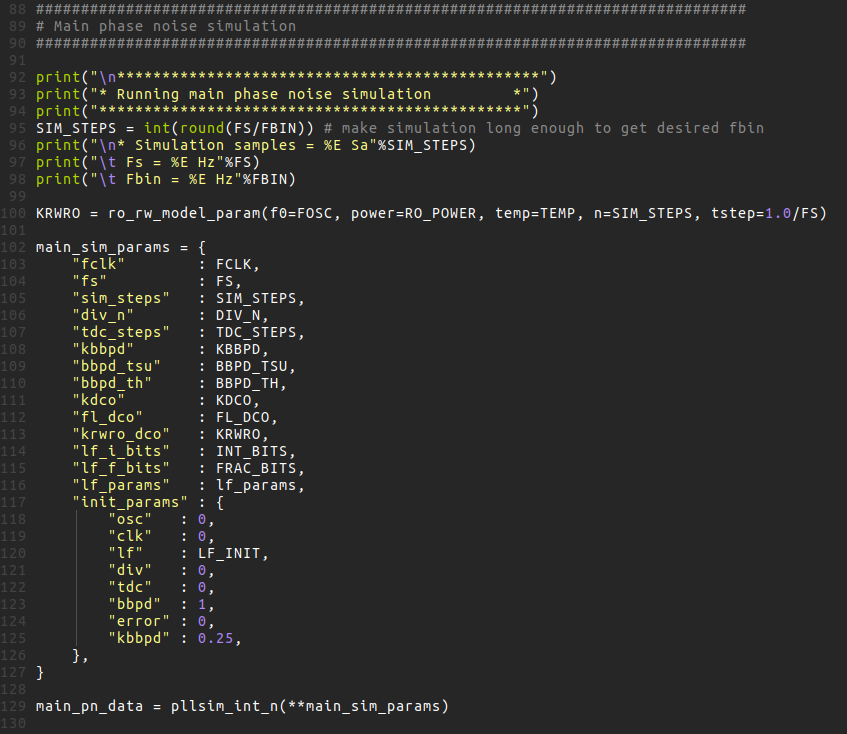
\includegraphics[width=0.45\textwidth, angle=0]{simulation_setup.png}
	\end{block}
\end{frame}




% #############################################################################
% Loop Dynamics (continuous)
% #############################################################################

% \begin{frame}
% 	\frametitle{Loop Dynamics}
% 	\begin{block}{Still To Do}
% 		\vspace{-.2em}
% 		\begin{itemize}
% 			\footnotesize
% 			\item Standard approach to used mixed continuous/discrete time mathematical model for DPLL. 
% 			\item Plot of RO phase noise (typical)
% 			\item Automatic analysis of performance (lock detection, residual phase modulation, lock-in/pull-in range).
% 			\item Automatic optimization (using gradient descent) of PLL parameters?
% 			\item Z-domain modeling of loop? Develop (by hand) some ideal transfer funtions for loop.

% 		\end{itemize}    
% 	\end{block}
% \end{frame}

% #############################################################################
% Specification
% #############################################################################

\begin{frame}
	\frametitle{Specification (unchanged)\color{black}}
	\begin{block}{System Performance Targets}
		\scriptsize
		\begin{table}[h!]
			\centering
			\def\arraystretch{1.5}		
			\setlength\arrayrulewidth{0.75pt}
			\setlength{\tabcolsep}{1em} % for the horizontal padding
			\begin{tabular}{|l|r|l|l|}
				\hline 
				\rule[-1ex]{0pt}{2.5ex} \cellcolor{gray!40}\textbf{Parameter} & \cellcolor{gray!40}\textbf{Value} & \cellcolor{gray!40}\textbf{Unit }& \cellcolor{gray!40}\textbf{Notes}\\ 
				\hline 
				\rule[-1ex]{0pt}{2.5ex} \textbf{Frequency}  & 2.4-2.4835 & GHz & 2.4G ISM Band\\ 
				\hline 
				\rule[-1ex]{0pt}{2.5ex} \textbf{Ref. frequency} & 16 & MHz & Yields 6 channels \\ 
				\hline 
				\rule[-1ex]{0pt}{2.5ex} \textbf{Power} & $\leq$ 100  &$\mu$W & \\ 
				\hline 
				\rule[-1ex]{0pt}{2.5ex} \textbf{FSK BER} & $\leq$ 1e-2  & & 2FSK with $f_{dev}$=$\pm$250 KHz\\ 
				\hline 
				\rule[-1ex]{0pt}{2.5ex} \textbf{Initial Lock Time} & $\leq$ 50 & $\mu$s & Upon cold start \\ 
				\hline 
				\rule[-1ex]{0pt}{2.5ex} \textbf{Re-lock Time} & $\leq$ 5 & $\mu$s & Coming out of standby \\ 
				\hline 
				\rule[-1ex]{0pt}{2.5ex} \textbf{Bandwidth} & 50 & kHz & (nominally), tunable \\ 
				\hline 
			\end{tabular} 
			% \caption{Assigned specifications for branch line hybrid design.}
			% \label{asgn_specs}
		\end{table}   
		Additionally: PLL output should support IQ sampling at LO frequency.
	\end{block}    
\end{frame}

\begin{frame}
	\frametitle{Specification (unchanged)}
	\begin{block}{PLL Component Performance Targets}
		\scriptsize
		\begin{table}[h!]
			\centering
			\def\arraystretch{1.5}		
			\setlength\arrayrulewidth{0.75pt}
			\setlength{\tabcolsep}{1em} % for the horizontal padding
			\begin{tabular}{|l|r|l|l|}
				\hline 
				\rule[-1ex]{0pt}{2.5ex} \cellcolor{gray!40}\textbf{Parameter} & \cellcolor{gray!40}\textbf{Value} & \cellcolor{gray!40}\textbf{Unit }& \cellcolor{gray!40}\textbf{Notes}\\ 
				\hline 
				\rule[-1ex]{0pt}{2.5ex} \textbf{DCO LSB Resolution}  & $\leq$ 50  & kHz & Determined from quantization noise.\\ 
				\hline 
				\rule[-1ex]{0pt}{2.5ex} \textbf{DCO DNL} & < 1 & LSB & Ensures monotonicity \\ 
				\hline 
				\rule[-1ex]{0pt}{2.5ex} \textbf{TDC Resolution} & 0.95  & ns & \\ 
				\hline 
				\rule[-1ex]{0pt}{2.5ex} \textbf{TDC Resolution (bits)} &  6 &bits & \\ 
				\hline 
			\end{tabular} 
			% \caption{Assigned specifications for branch line hybrid design.}
			% \label{asgn_specs}
		\end{table}   
	\end{block}    
\end{frame}

% #############################################################################
% Architecture - block diagram
% #############################################################################

\begin{frame}
	\frametitle{Architecture (updated)}
	\begin{block}{Block Diagram}
	\center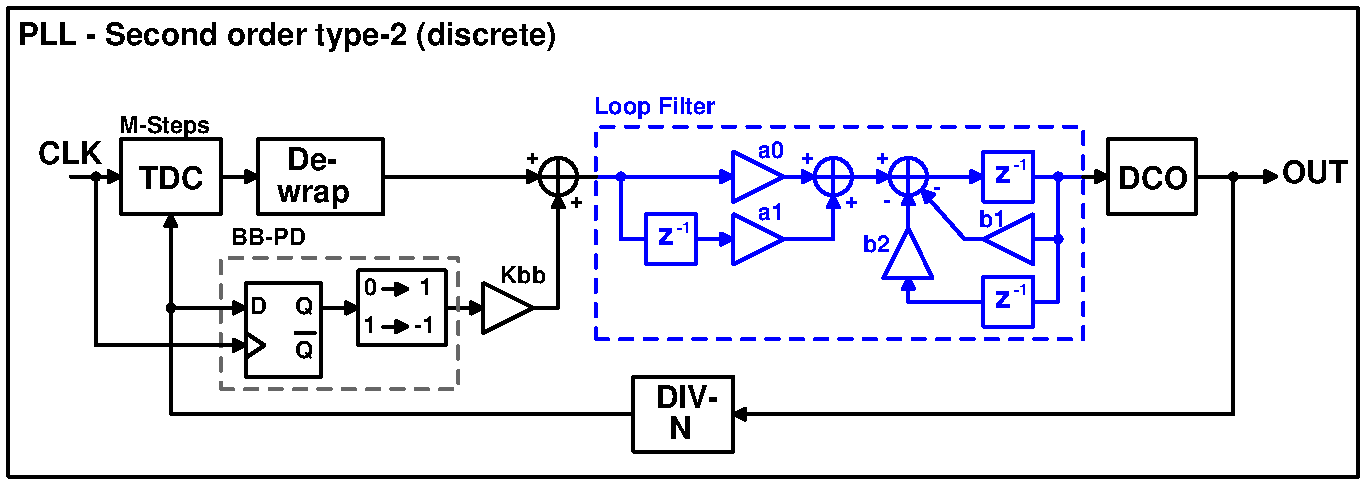
\includegraphics[width=0.8\textwidth, angle=0]{pll_sec_order_bb.pdf}

	\end{block}
		\begin{block}{Power Targets}
		\vspace{-.1em}
		\begin{table}[htb!]
			\tiny
			\centering
			\def\arraystretch{1.5}		
			\setlength\arrayrulewidth{0.75pt}
			\setlength{\tabcolsep}{1em} % for the horizontal padding
			\begin{tabular}{|l|l|l|l|l|}
				\hline 
				\rule[-1ex]{0pt}{2.5ex} \cellcolor{gray!40}\textbf{DCO} & \cellcolor{gray!40}\textbf{TDC} & \cellcolor{gray!40}\textbf{Divider }& \cellcolor{gray!40}\textbf{Other} & \cellcolor{gray!40}\textbf{SUM} \\ 
				\hline 
				\rule[-1ex]{0pt}{2.5ex} 70 $\mu$W& 20 $\mu$W & 10 $\mu$W & $<<$ 1 $\mu$W & 100 $\mu$W\\ 
				\hline 
			\end{tabular} 
			% \caption{Assigned specifications for branch line hybrid design.}
			% \label{asgn_specs}
		\end{table}   
	\end{block}

\end{frame}


% #############################################################################
% project phases
% #############################################################################


\begin{frame}
	\frametitle{Project Phases}
	\begin{block}{Autumn 2019}
		\footnotesize
		\begin{itemize}
			\item System modeling and simulation.
			\begin{itemize}
				\footnotesize
				\item Learn PLL theory in detail
				\item Evaluate feasability of PLL architectures (counter, TDC-based)
				\item Determine requirements for TDC/DCO/Divider/logic (bits of resolution, accuracy etc) to meet PLL performance specifications.
				\item Determine digital logic for loop filter, validate stability and lock time performance.
			\end{itemize}
			\item Research ultra-low power circuit topologies to implement system components that will meet determined requirements.
			\item Translate component-level specifications into schematic-level circuit designs.
			\begin{itemize}
				\footnotesize
				\item Try, fail, try again until functional at schematic level.
				\begin{itemize}
					\footnotesize
					\item I expect the TDC to be difficult.
				\end{itemize}
			\end{itemize}      
		\end{itemize}
	\end{block}
\end{frame}

% #############################################################################
% Project phases slide 2
% #############################################################################


\begin{frame}
	\frametitle{Project Phases (continued)}
	\begin{block}{Spring 2020}
		\begin{itemize}
			\footnotesize
			\item Finalize schematic-level design.
			\item Estabilish thorough tests for PLL performance (automated?) to help in layout.
			\item Layout of PLL.
			\begin{itemize}
				\footnotesize
				\item Design iteration until design specs met.
				\item Probably very time consuming.
			\end{itemize}
			\item Full characterization/validation of design performance. 
			\begin{itemize}
				\footnotesize
				\item Comprehensive Corners/Monte-Carlo testing (time consuming??)
				\item More design iteration if new issues crop up...
			\end{itemize}
			\item Thesis paper writing.
		\end{itemize}
	\end{block}
\end{frame}

% #############################################################################
% References
% #############################################################################


\begin{frame}
	\frametitle{References}
		\scriptsize
		[1] "Ultra-Low Power Wake-Up Receivers for Wireless Sensor Networks", N. Pletcher, J.M Rabaey, 2008.\\
		\hspace{16pt}\url{http://www.eecs.berkeley.edu/Pubs/TechRpts/2008/EECS-2008-59.html}\\
		\vspace{1em}
		% [2] "Minimum Achievable Phase Noise of RC Oscillators",
	% Navid et al. 2005
\end{frame}


\end{document}
